\documentclass[conference]{IEEEtran}
\IEEEoverridecommandlockouts
% \usepackage{cite}
\usepackage{verbatim}
\usepackage{amsmath,amssymb,amsfonts}
\usepackage{algorithmic}
\usepackage{graphicx}
\usepackage{textcomp}
\usepackage{xcolor}
\usepackage{amsmath,amsxtra,amsthm,amssymb,latexsym,wasysym}
\usepackage{textcomp,booktabs,multirow}
\usepackage{subfigure}
\usepackage[version=3]{mhchem}
\usepackage{chemarr}
\usepackage{lscape}
\usepackage{booktabs}
\newcommand{\chem}[1]{\ensuremath{\mathrm{#1}}}
\renewcommand\IEEEkeywordsname{Keywords}
\graphicspath{{Figure/}}
\graphicspath{{images/}}
\usepackage{float}
\usepackage{bookmark}
\usepackage{hyperref}
\usepackage{blindtext}
\usepackage{stfloats}
\usepackage{textgreek}
\usepackage{upgreek}
\usepackage{siunitx}
\usepackage{enumerate}
\usepackage{url}
\usepackage{threeparttable}
\usepackage[numbers, sort & compress]{natbib}
\def\BibTeX{{\rm B\kern-.05em{\sc i\kern-.025em b}\kern-.08em
    T\kern-.1667em\lower.7ex\hbox{E}\kern-.125emX}}

\title{Intrusion Detection of CAN Bus Attacks in Internet of Vehicles Using a Novel Machine Learning Approach}


\author{\IEEEauthorblockN{Aiman M. Reda}
\IEEEauthorblockA{Nile University\\Computer Science and Information Security\\
Giza, Egypt\\
a.mohamed2538@nu.edu.eg}
\and
\IEEEauthorblockN{Yasmin R. Shehab}
\IEEEauthorblockA{Nile University\\
Computer Science and Information Security\\
Giza, Egypt\\
Y.Ramadan2549@nu.edu.eg}
\and
\IEEEauthorblockN{Ahmed M. ElKhateeb}
\IEEEauthorblockA{Nile University\\
Computer Science and Informatics\\
Giza, Egypt\\
A.Mahmoud2440@nu.edu.eg}}


\begin{document}
\maketitle

\begin{abstract}
Modern vehicles communicate with each other via Internet of Vehicles (IoV) connectivity for synchronizing actions and preventing crashes for the safety of passengers and bystanders. IoV network packets are transmitted from signals that arise in the Controller Area Network (CAN) bus. However, those CAN signals may be prone to attacks such as Denial of Service (DoS), spoofing gas press, spoofing speed and wheel turns. In this study, we explore the nature of the CAN signals using the CiCIoV dataset, and propose a Machine Learning framework for detection of such cyberattacks. We conclude our study with addressing of an emerging problem of the hardship of detecting the replay attack in cars that use the same version of CAN signals as those collected inside the used dataset.
\end{abstract}

\begin{IEEEkeywords}
IoV, Cybersecurity, Machine Learning, Data Analysis
\end{IEEEkeywords}

The Internet of Vehicles (IoV) represents a transformative convergence of automotive engineering, wireless communication, and the Internet of Things (IoT), enabling vehicles to exchange data with one another, with roadside infrastructure, and with cloud-based services in real time \cite{inproceedings_fadhil}. Modern automobiles are no longer isolated mechanical systems; they are sophisticated cyber-physical platforms governed by over 100 Electronic Control Units (ECUs) that collectively manage safety-critical functions including engine control, anti-lock braking, airbag deployment, lane-keeping assistance, and adaptive cruise control \cite{article_enev_miro}. The global IoV market, valued at approximately USD 152 billion in 2024, is projected to surpass USD 755 billion by 2033 at a compound annual growth rate (CAGR) of 19.5\% \cite{article_abhijeet}, underscoring the accelerating pace of vehicular digitization and the growing dependence of transportation infrastructure on connected automotive systems.

At the heart of in-vehicle communication lies the Controller Area Network (CAN) bus protocol, originally developed by Bosch in the 1980s and subsequently standardized as ISO 11898 \cite{bosch1991can}. The CAN bus enables ECUs to exchange data over a shared two-wire broadcast bus at speeds of up to 1 Mbit/s, offering high reliability, low implementation cost, and strong resistance to electromagnetic interference \cite{szilagyi2014flexible}. Despite these engineering merits, the CAN protocol was designed in an era when vehicles were not externally networked and cybersecurity was not a design consideration. As a consequence, CAN lacks three fundamental security properties now considered essential in any networked communication system: sender authentication, message integrity verification, and payload encryption \cite{7429276}.

These architectural omissions create exploitable attack surfaces that grow more dangerous as vehicles gain external connectivity. Specifically, the absence of sender authentication means that any ECU — legitimate or malicious — can broadcast frames using any CAN identifier without challenge \cite{young2019canidssurvey}. The lack of encryption means all CAN frames are transmitted in plaintext, enabling eavesdropping, recording, and replay of sensitive vehicle data by any node with bus access \cite{10_1145_3431233}. The broadcast topology means a single compromised node can inject messages received simultaneously by every ECU on the bus, multiplying the impact of a single point of compromise \cite{article_avatefipour}. Modern vehicles further amplify these risks by incorporating multiple external communication interfaces — Wi-Fi, Bluetooth, 4G/5G cellular, and the OBD-II diagnostic port — each of which provides a potential remote entry point that adversaries may exploit to gain logical access to the CAN bus without physical proximity to the vehicle \cite{miller2015remote}.

Exploitation of CAN bus vulnerabilities has been demonstrated in numerous controlled security evaluations and real-world incidents. The principal attack categories include: Denial-of-Service (DoS) attacks, in which an adversary floods the bus with high-priority frames to prevent legitimate ECU communication; message spoofing attacks, in which falsified CAN frames manipulate vehicle sensor readings such as speed, engine RPM, gas pedal position, or steering wheel angle to induce incorrect actuator responses; fuzzing attacks, in which randomly generated frames are injected to probe for vulnerable ECU behaviors; and replay attacks, in which previously captured legitimate frames are retransmitted to trigger unintended vehicle actions \cite{s23073554}. The consequences range from driver inconvenience to catastrophic outcomes including loss of braking authority, unintended acceleration, and disabling of active safety systems, placing occupants, pedestrians, and road infrastructure at serious risk \cite{266537}. The automotive cybersecurity market, valued at USD 3.52 billion in 2024 and projected to reach USD 10.42 billion by 2034, reflects the urgency with which the industry is responding to these threats \cite{gmi2025automotivecybersecurity}.

Given the practical constraints of retrofitting authentication or encryption into deployed CAN networks — which would require coordinated updates across all ECUs and potentially affect real-time bus timing guarantees — Intrusion Detection Systems (IDS) have emerged as the primary defense strategy for in-vehicle network security \cite{7952095}. An IDS monitors CAN bus traffic continuously and raises alerts when anomalous or malicious patterns are identified, without modifying the underlying protocol. Machine learning (ML) has proven particularly well-suited to this task: ML models can learn complex, high-dimensional representations of normal and attack traffic from labeled CAN frame data, capturing both payload-level and temporal patterns that static rule-based systems would fail to generalize \cite{8476919}.

A broad range of ML algorithms has been applied to CAN bus IDS in the literature. Classical classifiers — Decision Trees (DT), Random Forests (RF), Logistic Regression (LR), and Support Vector Machines (SVM) — have demonstrated strong baseline performance on structured CAN frame data due to their interpretability, efficiency, and robustness to feature scaling \cite{8642311} [16, 23]. In particular, SVM has shown competitive detection accuracy across multiple vehicle datasets, benefiting from its maximum-margin classification boundary that generalizes well even when attack samples are scarce relative to benign traffic \cite{s23073610}. Deep learning architectures including Multilayer Perceptrons (DNN/MLP) and Convolutional Neural Networks (CNN) have been explored for their capacity to extract hierarchical representations from raw byte-level CAN data \cite{DESTA2022100470} [17, 24]. Ensemble methods combining multiple base classifiers have demonstrated further improvements in detection robustness, particularly for minority attack classes \cite{electronics14010069} [18, 20]. Dimensionality reduction techniques — Principal Component Analysis (PCA), Linear Discriminant Analysis (LDA), and the ANOVA F-test — have been applied to reduce feature space complexity and improve computational efficiency \cite{NABI2024100033} [19, 20].

Despite the volume of published work, a critical and frequently underemphasized challenge in CAN bus IDS research is data quality. Raw CAN bus captures are characterized by extreme redundancy: the CAN broadcast protocol causes ECUs to retransmit the same state data across consecutive frames, resulting in near-duplicate records that can constitute over 99\% of a dataset \cite{fi18010042}. When such duplicates are distributed across training and test splits without explicit removal, classifiers may effectively memorize repeated frames rather than learning generalizable attack patterns — a form of data leakage that produces inflated and non-reproducible performance metrics. Furthermore, the severe class imbalance inherent to real CAN traffic — where benign frames vastly outnumber attack frames — means that standard accuracy metrics can be misleading without complementary reporting of precision, recall, and F1-score per attack class. These data quality concerns motivate a rigorous data cleansing and Exploratory Data Analysis (EDA) pipeline as a mandatory precondition for trustworthy ML model evaluation: one that quantifies duplicate rates, characterizes per-class distributions, analyzes feature correlations, and addresses imbalance before any classifier is trained. In the present study, data cleansing and EDA are treated as first-class methodological contributions, not auxiliary preprocessing steps.

The CICIoV2024 dataset, released by the Canadian Institute for Cybersecurity, provides a realistic and richly labeled CAN bus traffic collection captured from a real vehicle under controlled attack conditions \cite{cic2024ciciov}. The dataset spans five attack categories — DoS and four spoofing variants targeting gas pedal position, RPM, vehicle speed, and steering wheel angle — alongside a large benign traffic baseline, encoded in binary, decimal, and hexadecimal formats. Recent studies on this dataset have produced important findings: Le and Alsmadi \cite{fi18010042} demonstrated that ANOVA-based feature selection preserves the integer-valued CAN payload structure that tree-based and SVM classifiers depend upon — a property that PCA-based reduction destroys — and that payload-identical Steering Wheel spoofing frames are indistinguishable from benign traffic without temporal features. Concurrently, Uddin et al. \cite{11098515} proposed a hierarchical three-level classification framework with SHAP-driven feature selection, achieving near-perfect detection rates. However, neither study provides a comprehensive benchmark incorporating SVM alongside deep learning models, nor a systematic EDA-grounded analysis of feature reduction strategies under consistent experimental conditions with explicit data cleansing.

The rest of this paper is organized as follows: Section \ref{sec:related_work} discusses the previous work in literature about the intrusion detection in IoV environments, section \ref{sec:Dataset_EDA} explores the hidden details of the used dataset and performing our preprocessing, section \ref{sec:architecture} proposed our novel ML architecture whose results are discussed in section \ref{sec:results}, finally we conclude our study in section \ref{sec:conclusion}.

\section{Related Work}
\label{sec:related_work}

The problem of intrusion detection in in-vehicle Controller Area Network (CAN) bus communication has attracted considerable research attention over the past decade. This section reviews the most relevant prior work, organized into four thematic areas: (1) classical machine learning approaches, (2) deep learning approaches, (3) ensemble and hybrid methods, and (4) data-centric approaches emphasizing preprocessing, exploratory data analysis (EDA), and feature selection. Table 1 summarizes the key studies reviewed.

\subsection{Classical Machine Learning Approaches}

Early ML-based IDS for CAN bus communication relied predominantly on classical supervised learning algorithms due to their interpretability, low computational requirements, and strong baseline performance on structured tabular data. Decision Trees (DT) and Random Forests (RF) were among the first classifiers applied to CAN bus anomaly detection, exploiting the tabular nature of CAN frame data — comprising an 11-bit identifier and up to 8 bytes of payload — which maps naturally to tree-based splitting criteria \cite{young2019canidssurvey}. Young et al. \cite{young2019canidssurvey} demonstrated that frequency-based features capturing the temporal regularity of CAN message identifiers provide significant discriminative power for DoS detection even with shallow classical models, a finding that informed subsequent feature engineering choices in the field.

A particularly influential study by Bari, Yelamarthi, and Ghafoor \cite{fi18010042} evaluated Support Vector Machine (SVM), Decision Tree, and K-Nearest Neighbor (KNN) classifiers on two real-world CAN bus datasets captured from a Kia Soul and a Chevrolet Spark. Their SVM-based IDS achieved detection accuracy up to 99.9\%, demonstrating SVM's effectiveness as a maximum-margin classifier even when class boundaries in CAN frame feature space are closely spaced. Their multi-dataset evaluation further highlighted a critical generalizability challenge: a model trained on one vehicle's CAN traffic may underperform on a different vehicle's network topology, motivating the need for rigorous dataset characterization and preprocessing before training. This finding directly supports the inclusion of SVM in the present study and underscores the importance of thorough EDA prior to model development.

Logistic Regression (LR) has been studied as a lightweight linear baseline for binary attack classification, offering fast inference suitable for resource-constrained in-vehicle hardware \cite{8642311}. However, its linear decision boundary limits performance on multi-class spoofing variants where class distributions in the feature space are non-linearly separable. Comparative evaluations have consistently shown that tree-based models outperform LR on raw CAN byte features, while SVM with a radial basis function (RBF) kernel offers a middle ground — capturing non-linear boundaries without the full representational overhead of deep learning \cite{fi18010042}.

\subsection{Deep Learning Approaches}

The growing availability of large-scale CAN bus datasets has facilitated the adoption of deep learning architectures capable of learning hierarchical representations from raw byte-level data. Convolutional Neural Networks (CNNs) have been applied to model local spatial patterns within CAN frame payloads, treating the 8-byte data field as a one-dimensional sequence amenable to convolutional feature extraction \cite{DESTA2022100470}.

Lo et al. \cite{11098515} proposed a hybrid CNN-LSTM deep learning framework that combines spatial feature extraction via convolution with temporal dependency modeling via Long Short-Term Memory (LSTM) units, improving detection of sequential attack patterns such as DoS floods and replay sequences on the Car-Hacking dataset. However, the increased model complexity introduces computational overhead that may be prohibitive for real-time deployment on automotive embedded systems with strict latency requirements. Ben Hassane et al. \cite{LO2022100471} evaluated LSTM and CNN models on two public datasets — Car-Hacking and CAN-Intrusion — and additionally on a self-generated simulation dataset produced using the ICSim tool, observing that LSTM models benefited from the sequential structure of CAN traffic but suffered performance degradation when the temporal window size was poorly calibrated.

Ahmed and Sharma \cite{s23073610} introduced an Attention-CNN-LSTM hybrid (ACL-IDS) incorporating a self-attention mechanism to dynamically weight the most informative time steps in a CAN message sequence, achieving state-of-the-art accuracy on the Car-Hacking dataset. Despite its strong performance, the authors acknowledged that the multi-layer attention mechanism substantially increases training and inference time, limiting practical deployment feasibility on constrained automotive hardware. Tüfekcioğlu, Hanilçi, and Gürkan \cite{article_taneja} addressed this limitation by proposing a lightweight CNN architecture optimized for embedded deployment, trading a marginal reduction in accuracy for a significant reduction in parameter count and inference latency. A recent study by Derhab et al. \cite{article_samir} evaluated Bidirectional LSTM (Bi-LSTM), GRU, and standard LSTM architectures on CAN datasets, finding that Bi-LSTM's ability to process sequences in both forward and backward temporal directions improved detection of attack onset boundaries — a property particularly relevant for spoofing attacks where the injected frame pattern emerges gradually.

A key limitation shared across all reviewed deep learning studies is their exclusive reliance on the Car-Hacking and OTIDS datasets, which were collected from older Hyundai vehicles (circa 2010–2016) and contain limited attack variety. No reviewed deep learning study has conducted a comprehensive benchmark on the CICIoV2024 dataset, which provides a broader and more recent attack taxonomy — a gap the present work addresses.

\subsection{Ensemble and Hybrid Methods}

Ensemble methods that combine multiple base classifiers have demonstrated consistent performance improvements over individual models in CAN bus IDS tasks, by reducing both variance through bagging and bias through boosting or stacking strategies. Random Forest itself constitutes a bagging ensemble of decision trees, and its strong performance across multiple studies [16, 25] has positioned it as a de facto benchmark for CAN bus classification.

Le and Alsmadi \cite{article_emre} constructed a voting ensemble of RF, DT, LR, DNN, and CNN classifiers on the CICIoV2024 dataset, demonstrating that ensemble voting improves F1-score for minority attack classes — particularly GAS spoofing and Steering Wheel spoofing — relative to any individual model. Their study is notable for explicitly addressing class imbalance and data redundancy in CICIoV2024, revealing that the near-perfect accuracy reported in several earlier studies is attributable to duplicate frame leakage across training and test sets rather than genuine model generalization. Their work does not, however, include SVM in the ensemble, nor does it provide a systematic three-way comparison of feature reduction strategies.

Uddin et al. \cite{article_rai} proposed a three-level hierarchical classification framework: the first level performs binary (attack/benign) detection, the second level identifies the attack category (DoS vs. spoofing), and the third level classifies the specific spoofing subtype. Using Boruta feature selection enhanced with SHAP-based explainability, their hierarchical ensemble achieved near-perfect detection rates on CICIoV2024. While architecturally compelling, the three-stage inference pipeline introduces latency that may conflict with real-time automotive IDS requirements. Moreover, their evaluation does not include SVM, does not compare PCA and LDA as alternative reduction strategies, and does not document a systematic data cleansing or EDA stage prior to model training.

\subsection{Data Cleansing, Exploratory Data Analysis, and Feature Selection}

A critical and frequently underemphasized aspect of ML-based CAN bus IDS research is the quality and representativeness of the training data. Raw CAN bus captures contain substantial redundancy: the CAN protocol's broadcast nature causes the same ECU states to be retransmitted across consecutive frames, resulting in near-duplicate records that can constitute over 99\% of a dataset \cite{article_emre}. When such duplicates are not explicitly identified and removed during preprocessing, train-test data leakage becomes a serious methodological concern — a classifier may memorize repeated frames rather than learning generalizable attack patterns, yielding inflated and non-reproducible performance metrics that overstate real-world detection capability.

Exploratory Data Analysis (EDA) is an essential precursor to model training in this domain. EDA on CAN bus data encompasses statistical description of feature distributions, class distribution analysis to quantify the degree of imbalance, byte-level correlation analysis to inform feature selection, and visualization of inter-class separability to motivate the choice of dimensionality reduction technique. Despite its importance, EDA is treated as a superficial step in most reviewed studies — limited to reporting sample counts and accuracy figures — rather than as a substantive methodological contribution. The present work elevates data cleansing and EDA to first-class methodological stages, systematically reporting duplicate rates, per-class sample statistics, feature correlation matrices, and class imbalance ratios before any model is trained.

On feature selection, three principal strategies have been applied to CAN bus data. Principal Component Analysis (PCA) is an unsupervised linear transformation projecting features onto orthogonal principal components of maximum variance. While effective for dimensionality reduction in many domains, Le and Alsmadi \cite{article_emre} demonstrated that PCA is poorly suited to CAN bus data: it converts the integer-valued CAN identifier and payload bytes into abstract linear combinations that lose their protocol-semantic meaning, causing F1-scores to drop dramatically for tree-based models and SVM. Linear Discriminant Analysis (LDA) is a supervised variant that maximizes inter-class separability while minimizing intra-class scatter, offering improved class discrimination relative to PCA when labeled data is available \cite{NABI2024100033}. ANOVA F-test-based feature selection operates as a filter method, ranking individual features by their statistical association with the class label and retaining those with the highest discriminative power without any feature transformation. Because ANOVA preserves original integer CAN feature values, it maintains the protocol-semantic properties that tree-based classifiers and SVM depend upon, making it the most effective reduction strategy for this domain \cite{article_emre}. The present study provides the first systematic three-way comparison of all three strategies under consistent experimental conditions.

Addressing class imbalance is equally critical. In the CICIoV2024 dataset, benign frames account for approximately 86.8\% of all records, while minor attack categories such as GAS spoofing represent less than 0.71\% of the total. A classifier predicting "benign" for every sample would achieve 86.8\% accuracy trivially, making accuracy an unreliable primary metric. The Synthetic Minority Over-sampling Technique (SMOTE) \cite{Chawla_2002} generates synthetic minority class samples by interpolating between existing instances in feature space, improving classifier sensitivity to rare attack patterns. Class-weighted loss functions offer an alternative by penalizing misclassification of minority classes more heavily during training without modifying the underlying data distribution \cite{electronics14010069}. Both strategies are considered in the present study and their effects reported per attack class.

\subsection{Research Gap and Positioning of This Work}

A synthesis of the reviewed literature reveals four unaddressed gaps that collectively motivate the present study. First, no existing work provides a comprehensive benchmark of classical ML (DT, RF, LR, SVM), deep learning (DNN/MLP, CNN), and ensemble methods on the CICIoV2024 dataset under consistent, reproducible experimental conditions — particularly with the inclusion of SVM, which has demonstrated competitive performance on real vehicle CAN data \cite{fi18010042} but has been excluded from all CICIoV2024 studies to date. Second, no study has conducted a systematic three-way comparison of PCA, LDA, and ANOVA as feature reduction strategies specifically for CAN bus IDS, with explicit per-class performance analysis across all attack types. Third, while the data quality issues of CICIoV2024 have been identified by Le and Alsmadi \cite{article_emre}, no subsequent study has incorporated thorough data cleansing and EDA as a formalized methodological stage with documented findings prior to model evaluation. Fourth, the novel model proposed in this work offers a technical contribution that advances beyond all reviewed baselines, motivated by and benchmarked against the comprehensive evaluation established through this study. Table 1 summarizes these distinctions.


\section{Dataset EDA}
\label{sec:Dataset_EDA}

This section presents a systematic Exploratory Data Analysis (EDA) of the
CICIoV2024 dataset, treated here as a first-class methodological stage rather
than auxiliary preprocessing. We characterize the dataset schema across its three
encodings, quantify data-quality issues (notably duplication and class
imbalance), and analyze the discriminative structure of the CAN identifier and
payload fields. All statistics reported below were computed on the full dataset
($N=1{,}408{,}219$ frames) using the decimal encoding unless otherwise stated.

\subsection{Dataset Composition and Schema}

The CICIoV2024 dataset is distributed in three numerically equivalent
encodings of the same captured CAN frames: \emph{decimal}, \emph{hexadecimal},
and \emph{binary}. Each encoding is organized as six label-pure CSV files, one
per traffic class (BENIGN, DoS, and the four spoofing variants GAS, RPM, SPEED,
and STEERING\_WHEEL). The decimal encoding represents each frame compactly as the
11-bit CAN identifier \texttt{ID} and eight payload bytes
\texttt{DATA\_0}--\texttt{DATA\_7} (each in $[0,255]$), followed by three label
columns (\texttt{label}, \texttt{category}, \texttt{specific\_class}). The
hexadecimal encoding additionally carries an \texttt{Interface} field (constant
\texttt{slcan0}) and a Data Length Code \texttt{DLC} (constant \texttt{[8]}),
both of which are zero-variance and therefore carry no discriminative
information; we further observe that the hexadecimal DoS file omits the
\texttt{DLC} column entirely. The binary encoding bit-explodes every field into
153 binary features. Table~\ref{tab:encoding_comparison} summarizes the three
encodings.

We verified that the encodings are exact re-expressions of the same data by
decoding a random sample of hexadecimal frames to integers and comparing them to
the corresponding decimal frames; the match rate was $1.0000$ for both the
identifier and the payload bytes. Because the decimal encoding preserves the
integer-valued, protocol-semantic structure of CAN frames with the smallest
feature count and no constant columns, we adopt it as the primary representation
for all subsequent analysis and modeling, consistent with the observation of Le
and Alsmadi~\cite{article_emre} that transformations destroying integer payload
semantics degrade tree-based and SVM performance.

\begin{table}[htbp]
\centering
\caption{Comparison of the three CICIoV2024 encodings.}
\label{tab:encoding_comparison}
\begin{tabular}{lccc}
\hline
Property & Decimal & Hexadecimal & Binary \\
\hline
Feature columns   & 9      & 9              & 153 \\
Requires parsing  & No     & Yes (hex)      & No \\
Constant columns  & None   & Interface, DLC & None \\
Information content & Full  & Identical      & Identical \\
Role in this study & Primary & Consistency  & Not used \\
\hline
\end{tabular}
\end{table}

\subsection{Class Distribution and Imbalance}

The dataset exhibits severe class imbalance. Benign traffic accounts for
$86.90\%$ of all frames, whereas the smallest attack class, GAS spoofing,
constitutes only $0.71\%$. The resulting imbalance ratio between the largest and
smallest classes is approximately $122.5{:}1$. Table~\ref{tab:class_distribution}
reports the per-class counts and proportions. This imbalance renders raw
accuracy an unreliable headline metric --- a trivial classifier predicting
``benign'' for every frame would attain $86.90\%$ accuracy --- and motivates our
use of class-weighted training together with per-class precision, recall, and
F1-score, and macro-averaged metrics in Section~\ref{sec:results}.

\begin{table}[htbp]
\centering
\caption{Per-class distribution of the CICIoV2024 dataset (decimal encoding, full data).}
\label{tab:class_distribution}
\begin{tabular}{lrr}
\hline
Class & Count & Percentage (\%) \\
\hline
BENIGN          & 1{,}223{,}737 & 86.900 \\
DoS             & 74{,}663      & 5.302 \\
GAS             & 9{,}991       & 0.709 \\
RPM             & 54{,}900      & 3.899 \\
SPEED           & 24{,}951      & 1.772 \\
STEERING\_WHEEL & 19{,}977      & 1.419 \\
\hline
Total           & 1{,}408{,}219 & 100.000 \\
\hline
\end{tabular}
\end{table}

\subsection{Data Redundancy and Leakage Risk}

Consistent with the broadcast nature of the CAN protocol, the dataset is
extremely redundant: $99.75\%$ of all frames ($1{,}404{,}631$ of $1{,}408{,}219$)
are exact duplicates of an earlier frame, and the entire dataset reduces to only
$3{,}588$ distinct feature-frames. Table~\ref{tab:unique_frames} decomposes this
redundancy by class. The attack classes are especially degenerate: GAS spoofing
comprises just $2$ unique frames repeated $9{,}991$ times, STEERING\_WHEEL $3$
frames, SPEED $5$, RPM $10$, and DoS $21$. In total, the four spoofing attacks
and DoS span only $41$ unique frames.

This degeneracy is the root cause of the inflated, near-perfect metrics reported
by several prior studies. Under a naive random train/test split, identical
copies of the same frame are distributed across both partitions, allowing a
classifier to memorize specific frames rather than learn generalizable attack
patterns --- a form of train/test data leakage~\cite{article_emre,fi18010042}.
We emphasize, however, that \emph{removing} duplicates is not an acceptable
remedy here, as it would collapse the attack data to $41$ rows and destroy the
class balance entirely. Instead, we recommend a \emph{group-aware} evaluation
protocol in which each unique frame defines a group assigned in its entirety to
either the training or the test partition, never both, thereby preserving the
data volume while eliminating leakage.

\begin{table}[htbp]
\centering
\caption{Total frames versus distinct feature-frames per class.}
\label{tab:unique_frames}
\begin{tabular}{lrr}
\hline
Class & Total frames & Unique frames \\
\hline
BENIGN          & 1{,}223{,}737 & 3{,}547 \\
DoS             & 74{,}663      & 21 \\
GAS             & 9{,}991       & 2 \\
RPM             & 54{,}900      & 10 \\
SPEED           & 24{,}951      & 5 \\
STEERING\_WHEEL & 19{,}977      & 3 \\
\hline
\end{tabular}
\end{table}

\subsection{CAN Identifier Analysis}

The CAN identifier alone is highly discriminative. Benign traffic spans $72$
distinct identifiers, whereas each attack class uses only one or two. Crucially,
\emph{none} of the attack identifiers overlaps with the benign identifier set:
DoS targets ID~$291$, GAS ID~$513$, RPM IDs~$\{476,513\}$, SPEED IDs~$\{344,
513\}$, and STEERING\_WHEEL ID~$128$, and the set intersection of each attack's
identifiers with the benign identifiers is empty. Consequently, an attack can be
distinguished from benign traffic on the basis of the identifier field alone,
which explains both the near-perfect separability of the dataset and the
suitability of lightweight classifiers. Figure~\ref{fig:can_id_heatmap}
visualizes the row-normalized frequency of the most common identifiers across
classes, in which each attack class activates its own distinct column(s).

\begin{figure}[htbp]
    \centering
    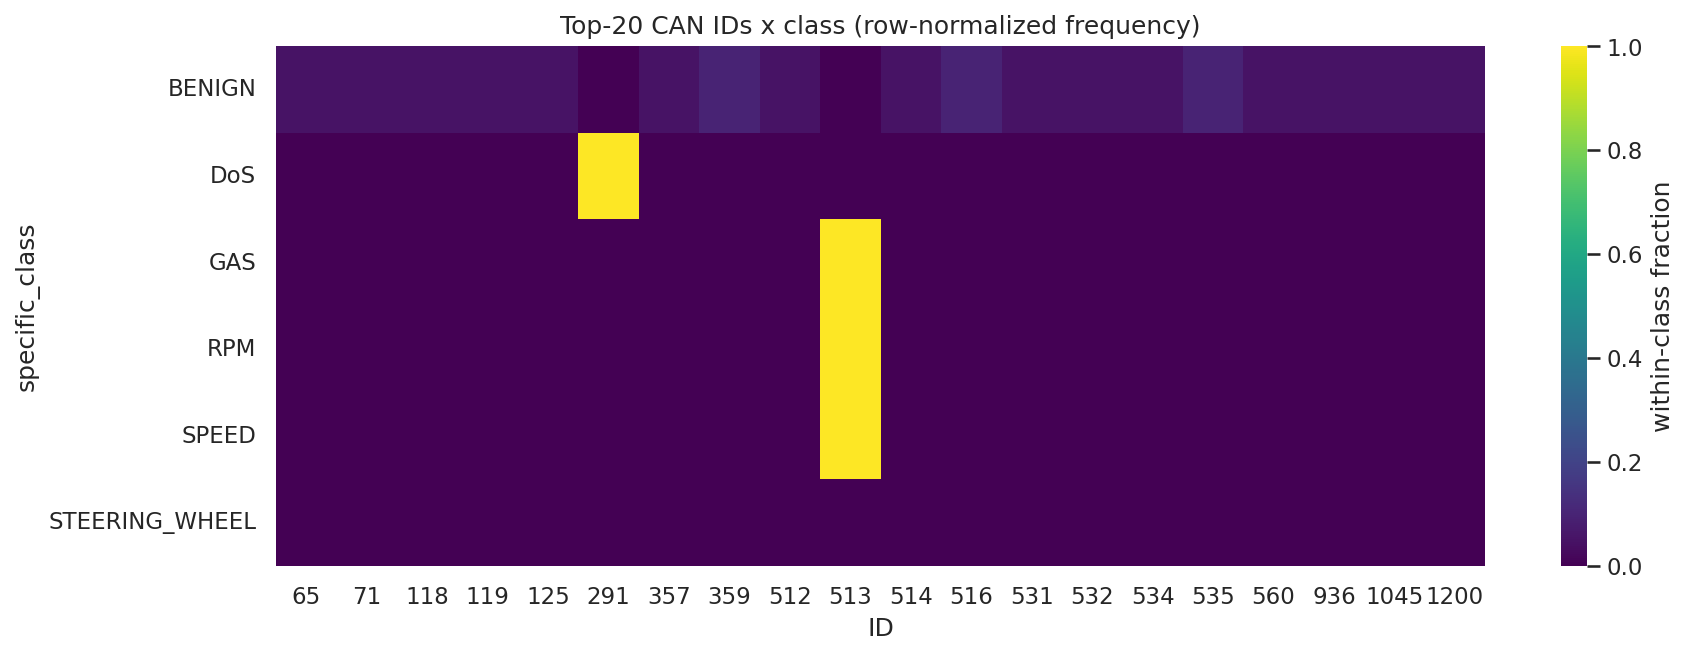
\includegraphics[width=1\linewidth]{can_id_class_heatmap.png}
    \caption{Row-normalized frequency of the top-20 CAN identifiers across
    classes. Each attack class concentrates on identifiers disjoint from benign
    traffic.}
    \label{fig:can_id_heatmap}
\end{figure}

\subsection{Payload Analysis}

Analysis of the eight payload bytes corroborates the separability observed in the
identifier field. We quantify the variability of each byte per class using
Shannon entropy $H = -\sum_i p_i \log_2 p_i$, where $p_i$ is the empirical
probability of byte value $i$; $H=0$ indicates a perfectly constant byte and
$H=8$ a uniformly distributed one. Attack payloads exhibit markedly low entropy
relative to benign traffic: all six payload bytes of GAS spoofing are constant
($H\approx 0$) except the final two, and STEERING\_WHEEL is constant in six of
eight bytes. Benign traffic, by contrast, shows substantially higher and more
uniform entropy across bytes. Figure~\ref{fig:payload_entropy} presents the
per-byte entropy heatmap, and Figure~\ref{fig:payload_dist} the per-byte value
distributions by class.

We deliberately omit a byte-to-byte correlation analysis: CAN payload bytes
encode unrelated physical signals and checksums, so cross-byte correlation is not
expected to be informative for this dataset.

\begin{figure}[htbp]
    \centering
    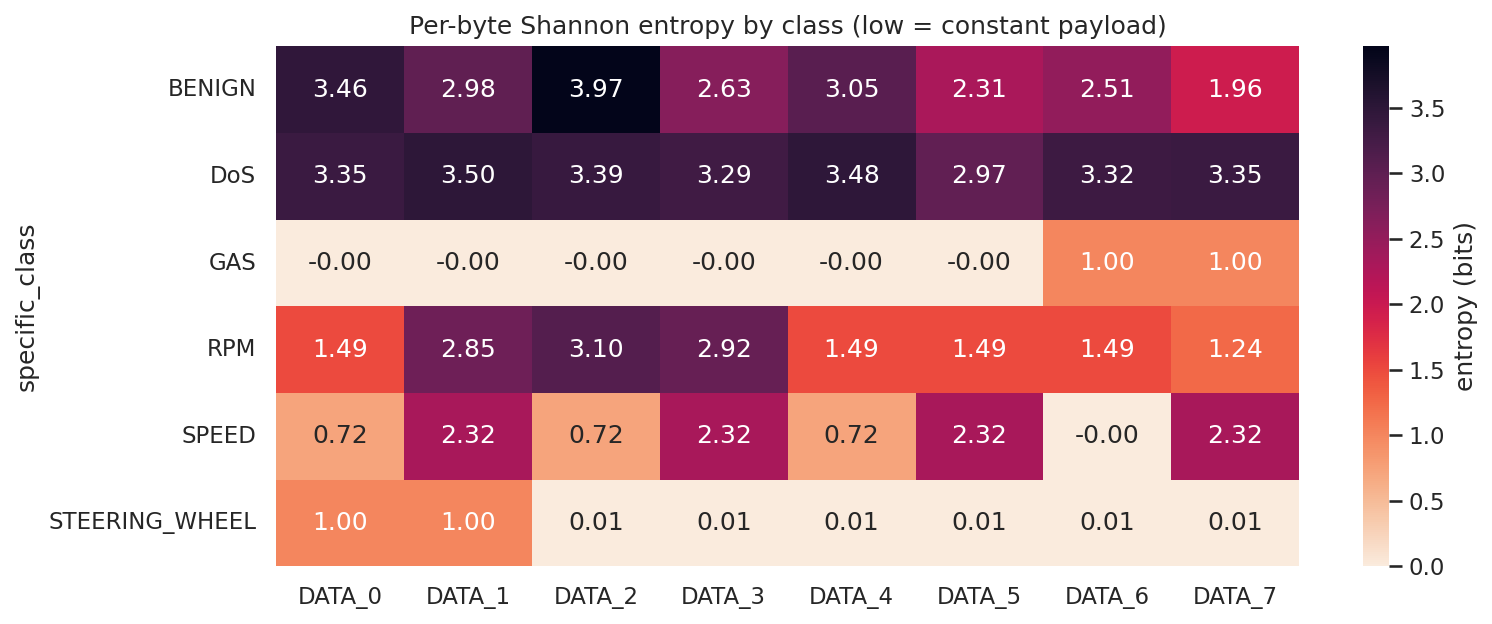
\includegraphics[width=1\linewidth]{payload_entropy_heatmap.png}
    \caption{Per-byte Shannon entropy (bits) by class. Low values indicate
    constant, injected payloads characteristic of the spoofing attacks.}
    \label{fig:payload_entropy}
\end{figure}

\begin{figure}[htbp]
    \centering
    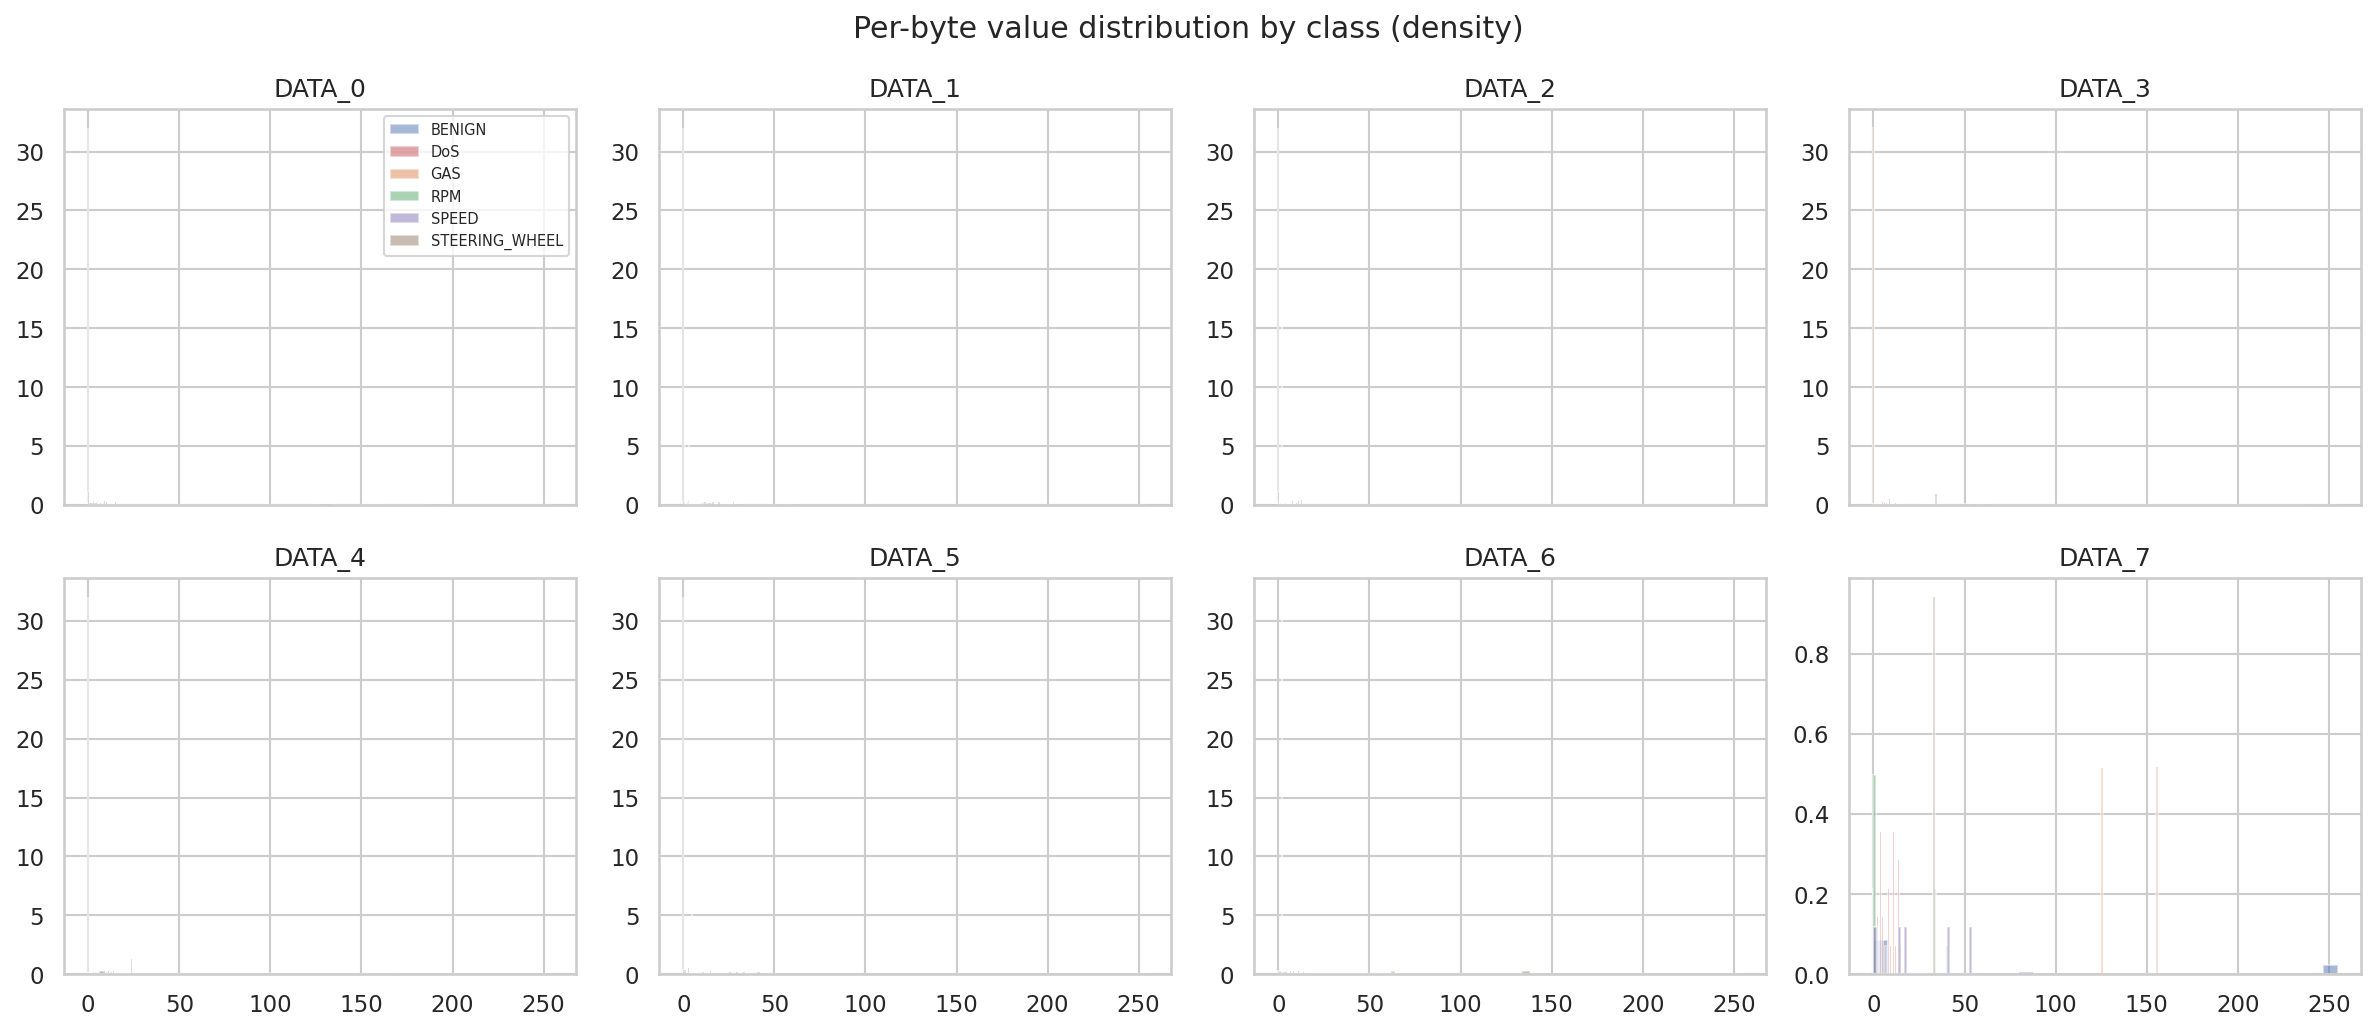
\includegraphics[width=1\linewidth]{payload_byte_distributions.png}
    \caption{Per-byte payload value distributions by class (density-normalized).}
    \label{fig:payload_dist}
\end{figure}

Finally, Table~\ref{tab:attack_signatures} reports a compact signature for each
attack: its targeted identifier, its single most frequent payload, and the share
of that payload among the attack's frames. For GAS and STEERING\_WHEEL, a single
frame accounts for half of all frames in the class, underscoring the highly
repetitive nature of these injections.

\begin{table}[htbp]
\centering
\caption{Dominant signature of each attack class (targeted ID, most frequent payload, and its share of class frames).}
\label{tab:attack_signatures}
\begin{tabular}{lcl c}
\hline
Class & ID & Most frequent payload & Share \\
\hline
DoS             & 291 & [3,3,0,9,7,3,7,4]      & 0.067 \\
GAS             & 513 & [0,0,0,0,0,0,64,156]   & 0.500 \\
RPM             & 476 & [2,61,23,19,0,0,0,0]   & 0.182 \\
SPEED           & 344 & [6,16,6,54,6,29,2,14]  & 0.200 \\
STEERING\_WHEEL & 128 & [132,3,2,35,24,5,138,34] & 0.500 \\
\hline
\end{tabular}
\end{table}

\subsection{EDA Summary}

The EDA establishes four findings that directly shape our methodology. First, the
three encodings are numerically equivalent, and the decimal encoding is the most
appropriate representation as it preserves integer CAN semantics with no constant
columns. Second, the dataset is severely imbalanced ($122.5{:}1$), mandating
per-class and macro-averaged evaluation. Third, $99.75\%$ of frames are
duplicates and the attacks span only $41$ unique frames, creating a substantial
leakage risk that we address through a group-aware split rather than duplicate
removal. Fourth, the dataset is near-perfectly separable: each attack uses CAN
identifiers disjoint from benign traffic and injects low-entropy, near-constant
payloads. This separability justifies our choice of lightweight classical
classifiers in Section~\ref{sec:architecture}.

\section{Architecture}
\label{sec:architecture}
We propose the usage of ML models for their lightweight computational requirements, as those models will be installed on the edge car which may not necessarily fulfill the requirements for the more resource intensive deep learning models.
Since the dataset is proven to be easily separable in section \ref{sec:Dataset_EDA}, we propose the usage of simply ML models which are SVM, Random Forest and XGBoost.
\subsection{Support Vector Machine (SVM)}
A Support Vector Machine of radial basis function (RBF) kernel was used and trained on the dataset with degree of 3 and decision function shape of One-Versus-Rest (ovr).
The entire pipeline is shown in figure \ref{fig:SVM_arch}
\begin{figure}
    \centering
    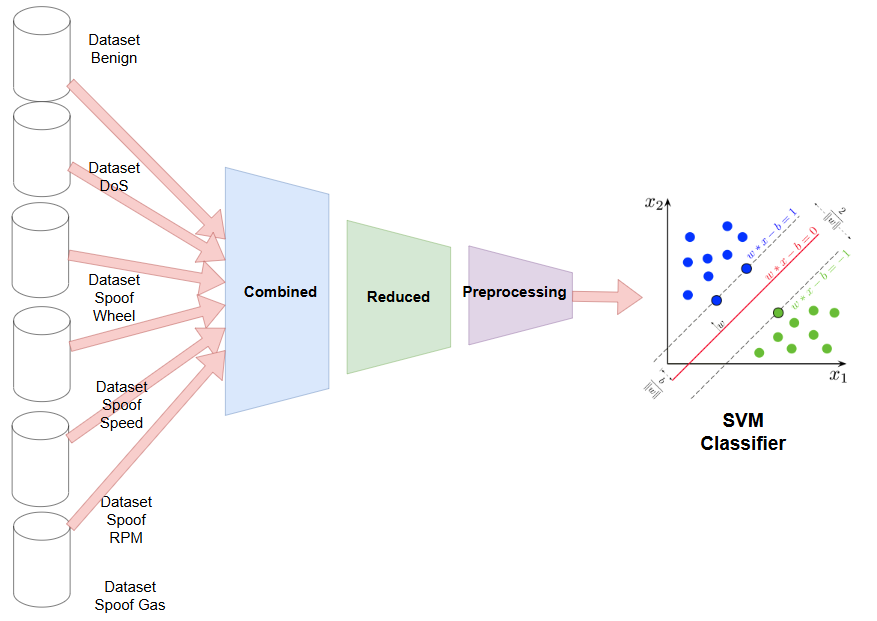
\includegraphics[width=1\linewidth]{SVM_arch.png}
    \caption{SVM training pipeline}
    \label{fig:SVM_arch}
\end{figure}
The dataset was split into 70\% for training and 30\% for testing. Training took relatively long time due to the vast size of the dataset.

\subsection{Random Forest}
Random Forest (RF) classifier is a famous ensemble bagging model that can combat excessive noise and variance in the dataset, it is also robust against human errors during annotation since it relies on different classifiers and takes the majority vote.
A random forest was created with gini criterion and number of estimators of 100 decision trees, training took an average of 67 seconds on the same machine discussed before.
Results of the used RF classifier for binary classification are discussed in section \ref{sec:results}

\subsection{XGBoost}
We trained an XGBoost classifier to see the effect of boosting on the dataset as we have previously tried the bagging model which is the Random Forest.
An XGBoost model was trained  using 10 estimators with a Decision Tree kernel.
The general architecture is shown in figure \ref{fig:XGBoost_Arch}
\begin{figure}
    \centering
    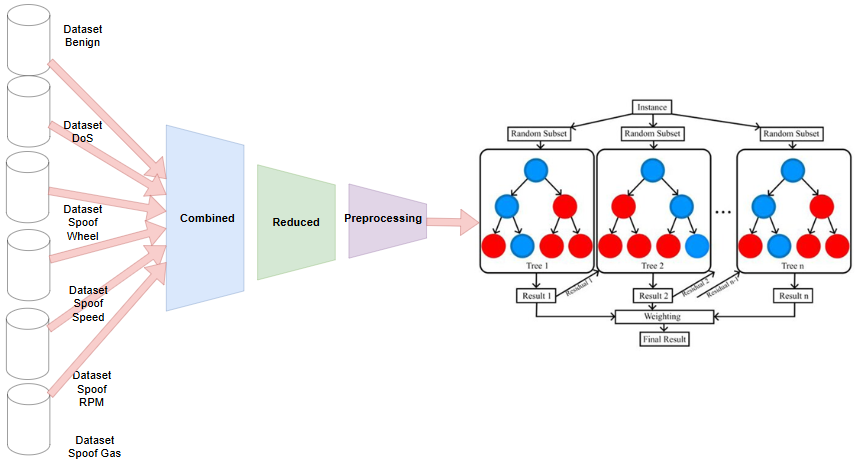
\includegraphics[width=1\linewidth]{XGBoost_Arch.png}
    \caption{Training Pipeline of the XGBoost classifier}
    \label{fig:XGBoost_Arch}
\end{figure}

\section{Results}
\label{sec:results}
\subsection{Evaluating the SVM}
SVM was trained according to the architecture in \ref{sec:architecture}, training was done on a machine equipped with Intel Core I7 10th Gen and 16GB of RAM, training was done via the CPU.
Training was performed twice, one run for the binary classification and the other for the classful classification, training time took 45.08 and 44.06 seconds respectively.
The classification metrics for the classful classification are shown in table \ref{tab:classification_report_svm} while the classification metrics for the binary classification are shown in table \ref{tab:svm_comparison_binary}

\begin{table}[h]
\centering
\caption{SVM multiclass Classification Report}
\begin{tabular}{lcccc}
\hline
\textbf{Class} & \textbf{Precision} & \textbf{Recall} & \textbf{F1-Score} & \textbf{Support} \\
\hline
BENIGN          & 0.999989 & 0.999542 & 0.999766 & 367122 \\
DoS             & 1.000000 & 1.000000 & 1.000000 & 22399 \\
GAS             & 1.000000 & 1.000000 & 1.000000 & 2997 \\
RPM             & 1.000000 & 0.908682 & 0.952157 & 16470 \\
SPEED           & 0.817497 & 1.000000 & 0.899585 & 7485 \\
STEERING\_WHEEL & 1.000000 & 0.999499 & 0.999750 & 5993 \\
\hline
Accuracy     & \multicolumn{3}{c}{0.996035} & 422466 \\
Macro Avg    & 0.969581 & 0.984621 & 0.975210 & 422466 \\
Weighted Avg & 0.996757 & 0.996035 & 0.996149 & 422466 \\
\hline
\end{tabular}
\label{tab:classification_report_svm}
\end{table}




\subsection{Evaluating the Random Forest}
\begin{table}[h]
\centering
\caption{Classification Report for the binary Random Forest Classifier}
\begin{tabular}{lcccc}
\hline
\textbf{Class} & \textbf{Precision} & \textbf{Recall} & \textbf{F1-Score} & \textbf{Support} \\
\hline
ATTACK       & 1.000000 & 0.999928 & 0.999964 & 55345  \\
BENIGN       & 0.999989 & 1.000000 & 0.999995 & 367121 \\
\hline
Accuracy     & \multicolumn{3}{c}{0.999991} & 422466 \\
Macro Avg    & 0.999995 & 0.999964 & 0.999979 & 422466 \\
Weighted Avg & 0.999991 & 0.999991 & 0.999991 & 422466 \\
\hline
\end{tabular}
\label{tab:classification_report_binary_rf}
\end{table}
The results for the RF classifier do not indicate the suspicious 100\% separability, indicating that the data was prone to data leakage or overtraining in the SVM classifier.
RF classifier was evaluated with its results in table \ref{tab:classification_report_binary_rf} for binary classification and in table \ref{tab:classification_report_multiclass_RF} for classful classification.

\begin{table}[h]
\centering
\caption{Classification Report for multiclass RF classifier}
\begin{tabular}{lcccc}
\hline
\textbf{Class} & \textbf{Precision} & \textbf{Recall} & \textbf{F1-Score} & \textbf{Support} \\
\hline
BENIGN          & 0.999989 & 1.000000 & 0.999995 & 367122 \\
DoS             & 1.000000 & 1.000000 & 1.000000 & 22399 \\
GAS             & 1.000000 & 1.000000 & 1.000000 & 2997 \\
RPM             & 0.915860 & 0.999939 & 0.956055 & 16470 \\
SPEED           & 1.000000 & 0.797862 & 0.887568 & 7485 \\
STEERING\_WHEEL & 1.000000 & 0.999499 & 0.999750 & 5993 \\
\hline
Accuracy     & \multicolumn{3}{c}{0.996409} & 422466 \\
Macro Avg    & 0.985975 & 0.966217 & 0.973894 & 422466 \\
Weighted Avg & 0.996710 & 0.996409 & 0.996286 & 422466 \\
\hline
\end{tabular}
\label{tab:classification_report_multiclass_RF}
\end{table}

\subsection{Evaluating the XGBoost}
Using the same training setup and the same machine. Binary XGBoost was trained and tested and output results in table \ref{tab:binary_classification_report_XGB}. The classful XGBoost was trained and tested and output results in table \ref{tab:multiclass_classification_report_XGB}

\begin{table}[htbp]
\centering
\caption{Detailed Classification Report of the Binary XGBoost Classifier}
\label{tab:binary_classification_report_XGB}
\begin{tabular}{lcccc}
\hline
Class & Precision & Recall & F1-Score & Support \\
\hline
ATTACK & 1.000000 & 0.999928 & 0.999964 & 55345 \\
BENIGN & 0.999989 & 1.000000 & 0.999995 & 367121 \\
\hline
Accuracy     & --       & --       & 0.999991 & 422466 \\
Macro Avg    & 0.999995 & 0.999964 & 0.999979 & 422466 \\
Weighted Avg & 0.999991 & 0.999991 & 0.999991 & 422466 \\
\hline
\end{tabular}
\end{table}

\begin{table}[htbp]
\centering
\caption{Detailed Classification Report of the Multiclass XGBoost Classifier}
\label{tab:multiclass_classification_report_XGB}
\begin{tabular}{lcccc}
\toprule
Class & Precision & Recall & F1-Score & Support \\
\midrule
BENIGN          & 0.999989 & 1.000000 & 0.999995 & 367122 \\
DoS             & 1.000000 & 1.000000 & 1.000000 & 22399 \\
GAS             & 1.000000 & 1.000000 & 1.000000 & 2997 \\
RPM             & 0.915860 & 0.999939 & 0.956055 & 16470 \\
SPEED           & 1.000000 & 0.797862 & 0.887568 & 7485 \\
STEERING\_WHEEL & 1.000000 & 0.999499 & 0.999750 & 5993 \\
\midrule
Accuracy     & --       & --       & 0.996409 & 422466 \\
Macro Avg    & 0.985975 & 0.966217 & 0.973894 & 422466 \\
Weighted Avg & 0.996710 & 0.996409 & 0.996286 & 422466 \\
\bottomrule
\end{tabular}
\end{table}


\section{Conclusion and Future Work}
\label{sec:conclusion}
In this study, we address the criticality of securing IoV communications in today's world, as well as address problems in the collected CiCIoV dataset. We propose different ML approaches to detect different intrusion techniques on the CAN bus of vehicles compromising the IoV communication. Results show that the XGBoost classifier is the most suitable given its inference speed and detection accuracy while being as lightweight as possible to be installed on the ECUs of vehicles. We conclude our study by proposing different collection points of the IoV packets to include 1- Timestamp, 2- Device Identifier, 3- Verifiable Signature tied with a challenge and 4- the CAN packet encrypted. The point of collection that has this much information is at the endpoint ECU itself and not the CAN bus. Future research should address the criticality of collecting information-rich datasets to allow proper training and ensure confidentiality and authentication of Intra-vehicle communication while being robust against DoS achieving unhindered availability.

\bibliographystyle{IEEEtran}
\bibliography{references}
\end{document}